\chapter{Introduction} \label{chap:intro}

%\section*{}

This chapter aims at giving a general overview about the themes addressed by this thesis. We will address the context in which the thesis is inserted, as well as the motivation that led to its proposal. Furthermore there will be a brief description of the main objectives of this thesis, and the methods that will be used to achieve those objectives.

\section{Context} \label{sec:context}

Web applications are getting more and more important. Due to their stability and security against losing data, there is a growing trend to move applications towards the Web, with the most notorious examples being Google's mail and office software applications. Web applications can now handle tasks that before could only be performed by desktop applications \cite{garrett2005ajax}, like editing images or creating spreadsheet documents.

Despite the relevance that Web applications have in the community, they still suffer from a lack of standards and conventions \cite{constantine2002usage}, unlike desktop and mobile applications. This means that the same task can be implemented in many different ways, which makes automated testing difficult to accomplish and inhibits reuse of testing code.

GUIs \textit{(Graphical User Interfaces)} of all kinds are populated with recurring behaviours that vary slightly. For example, authentication \textit{(login/password)} is a common behaviour in many software applications. However, the implementation of those behaviours may vary significantly. For a login, in some cases an error message may appear when the authentication fails; in others, the software application simply erases the inserted data and doesn't send a message to the user. These behaviours (patterns) are called User Interface (UI) patterns \cite{van2001patterns} and are recurring solutions that solve common design problems. Due to their widespread use, UI patterns allow users a sense of familiarity and comfort when using applications.

\section{Motivation and Objectives} \label{sec:goals}
This thesis is part of an investigation project named PBGT \textit{(Pattern-based GUI Testing)} \cite{moreira2013pattern}. The goal of this investigation project is to develop a model-based GUI testing tool and approach, usable as an industrial tool. This project has five parts: a DSL \textit{(Domain Specific Language)} named \textbf{PARADIGM} to define GUI testing models based on UI patterns; a modelation and testing environment, named \textbf{PARADIGM-ME}, made to support the creation of test models; an automatic test case generation tool, named \textbf{PARADIGM-TG}, that generates test cases from test models defined in PARADIGM; a test case execution tool, named \textbf{PARADIGM-TE}, which executes test cases, analyzes their coverage, and returns detailed execution reports; and finally \textbf{PARADIGM-RE}, a Web application reverse engineering tool whose purpose is to extract UI patterns from Web pages without access to their source code, and use the extracted patterns to generate a test model defined in PARADIGM. 

The relationship between the different components can be better understood in Figure \ref{fig:pbgt}. The activities (rounded corner rectangles) with the human figure mean that they are not fully automatic requiring manual intervention. The activities with the cog mean that part (or all) of that activity is automatic. The numbers within the activities define their sequencing.

\begin{figure}[htb]
  \begin{center}
    \leavevmode
    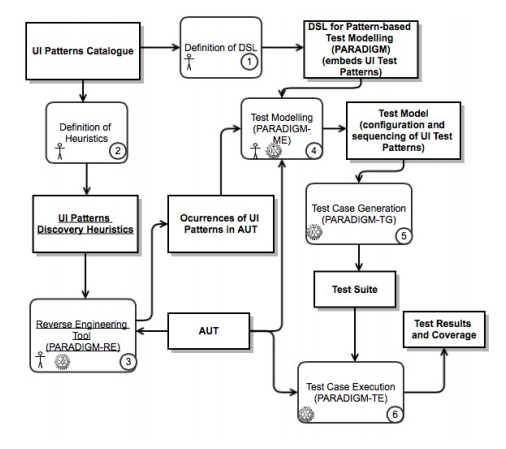
\includegraphics[width=0.8\textwidth]{pbgt}
  	\caption{An overview of the PBGT project \cite{nabuco2013inferring}}
  	\label{fig:pbgt}
   \end{center}
\end{figure}

The proposal aims to continue the work done on PARADIGM-RE \cite{nabuco2013inferring}. This tool identifies interface patterns using Machine Learning inference with the Aleph ILP system \footnote{Aleph: http://www.cs.ox.ac.uk/activities/machlearn/Aleph/aleph\_toc.html}. The tool was extended in \cite{nabuco2014inferring}, introducing a 

Considering the problem described and the proposed solution, the main goal for this research work is

\section{Expected Contributions} \label{sec:project}


\section{Structure of the Report} \label{sec:outline}

This document is structured into four main chapters. In this first section, Chapter \ref{chap:intro}, we start by introducing the theme to be developed during the course of the dissertation, starting by defining the context and issue at hand and describing the goals of this thesis.

Chapter \ref{chap:sota} introduces essential concepts to understand the problems with which this document deals, presents the state of the art of approaches that reverse-engineer Web applications, and lastly, gives some insight about data mining algorithms and how they will be applied to this work.

Chapter \ref{chap:approach} explains the solution proposed to the problem at hand. This chapter itself is also divided into several sections. First, to give a better understanding on the context in which the tool to develop will be implemented, a brief overview of the PARADIGM-RE tool is provided. Following this exposition, one then explains the approaches the author is considering to take, although these might be subject to change as the work progresses.

Chapter \ref{chap:workplan} outlines the main steps in the development of this thesis (and the respective software prototype) and attempts to provide a feasible schedule for the execution of the work to be done.

Chapter \ref{chap:conclusions} sums up the what has been defined in the report, emphasizing the problem that the thesis addresses and the work that will be executed towards solving that problem. It will also give a brief idea of what are the expected results at the end of the project.